\documentclass[11pt]{article}
\usepackage[margin=1in]{geometry}
\usepackage{graphicx}
\usepackage{listings}
\usepackage{xcolor}
\usepackage{verbatim}

\title{Functional Coverage Testing Report}
\author{}
\date{}

\begin{document}
\maketitle

\textbf{Project Structure}

The project follows a layered verification architecture with the following directory structure:

\begin{verbatim}
C:.
├───.git
├───docs
├───dut
├───funct_cov
│   └───delivery
│       ├───AN.DB
│       ├───csrc
│       ├───DVEfiles
│       ├───simv.daidir
│       └───simv.vdb
├───results
│   ├───coverage
│   └───logs
├───scripts
├───tb
└───tests
\end{verbatim}

\textbf{Layered Architecture Implementation}

A layered testbench architecture was implemented for the black box register controller design. The architecture includes transaction objects with randomized stimulus generation, Generator class connected to Driver, Monitor and Checker classes, and a dedicated Coverage component with functional coverage covergroups that monitors transactions through mailbox connections.

\textbf{Initial Testing Approach}

Initially, constraint-random testing was attempted but encountered errors. The approach was simplified to focus on basic read and write operations to establish a baseline functionality before adding complexity.

\begin{figure}[h]
\centering
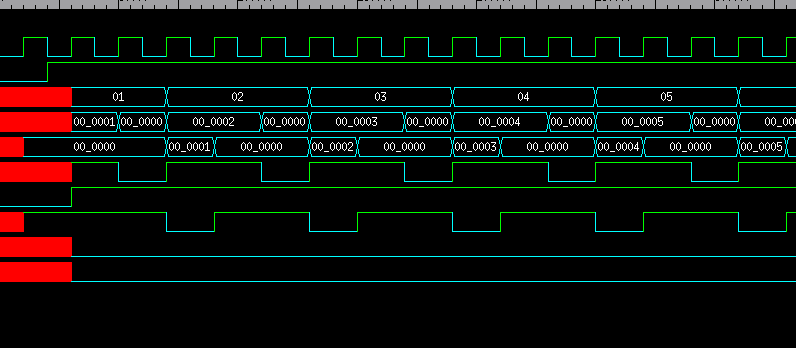
\includegraphics[width=0.8\textwidth]{normal_read_write.png}
\caption{Normal read and write operations testing}
\end{figure}

\textbf{Scoreboard Issues and Resolution}

During testing, errors were discovered in the scoreboard implementation. These were identified and corrected to ensure proper transaction verification and data integrity checking.

\textbf{Accumulate Functionality Bugs}

Several bugs were discovered in the accumulate functionality:

When acc=1 and func=1 (accumulate multiply), the design exhibited incorrect behavior:

\begin{figure}[h]
\centering
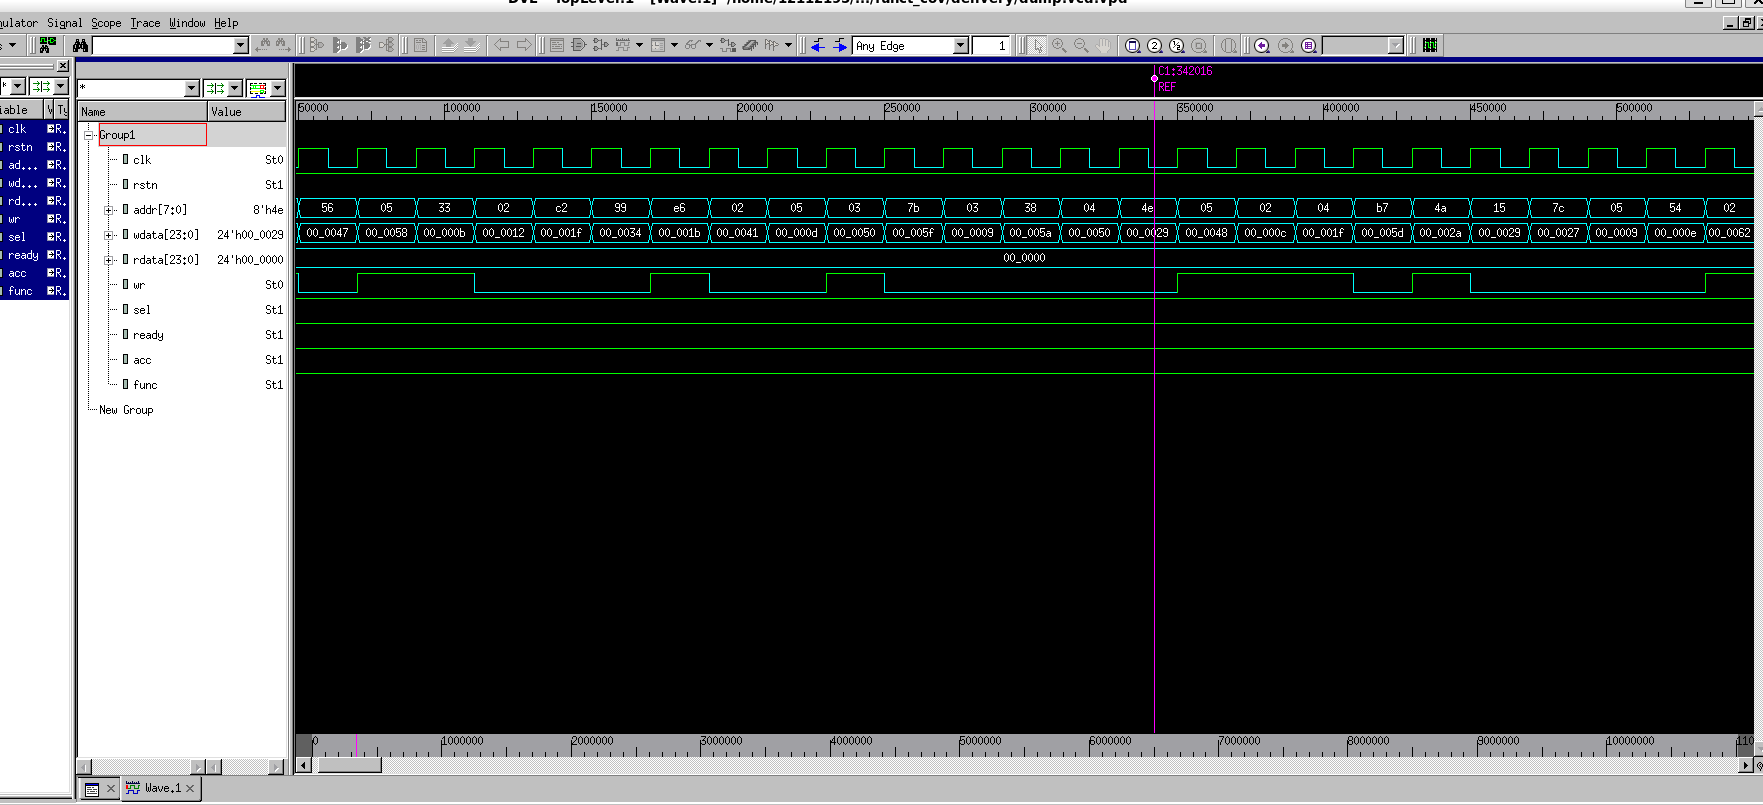
\includegraphics[width=0.8\textwidth]{acc_high_func_high_bug.png}
\caption{Bug discovered with acc=1, func=1 configuration}
\end{figure}

When acc=1 and func=0 (accumulate add), multiple issues were identified:

\begin{figure}[h]
\centering
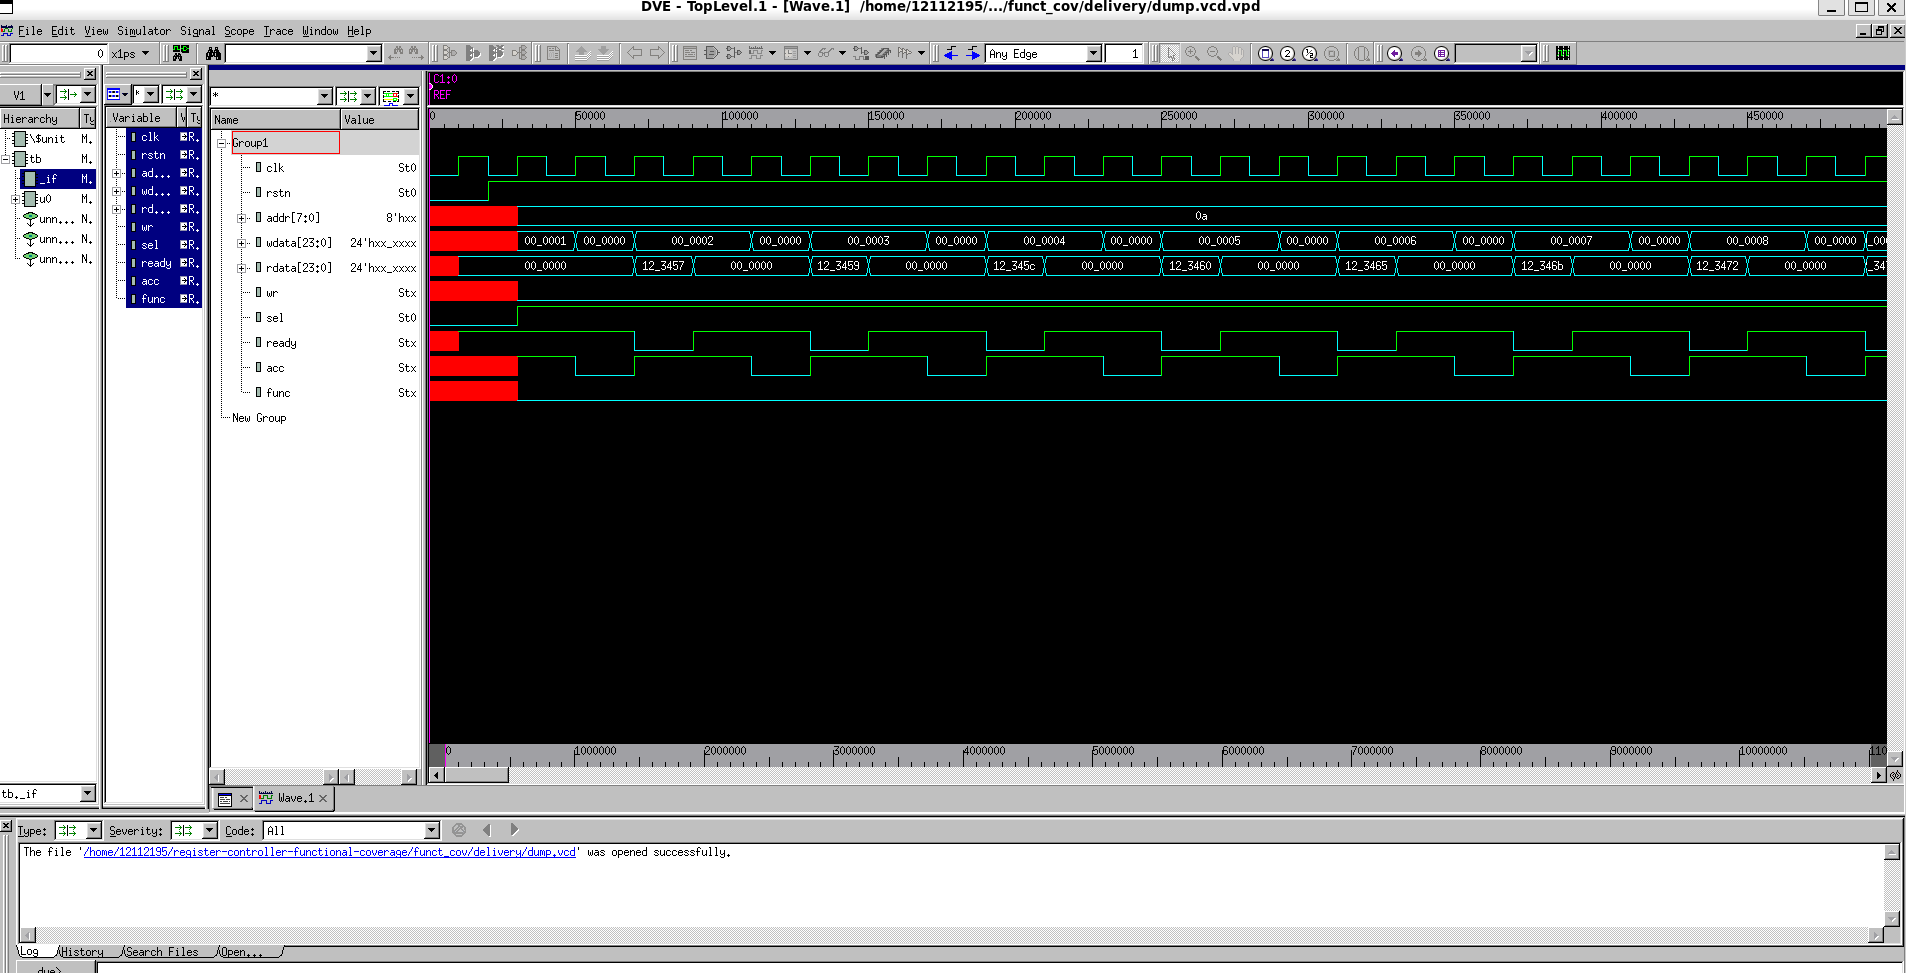
\includegraphics[width=0.8\textwidth]{acc_high_func_low_bug.png}
\caption{First bug with acc=1, func=0 configuration}
\end{figure}

\begin{figure}[h]
\centering
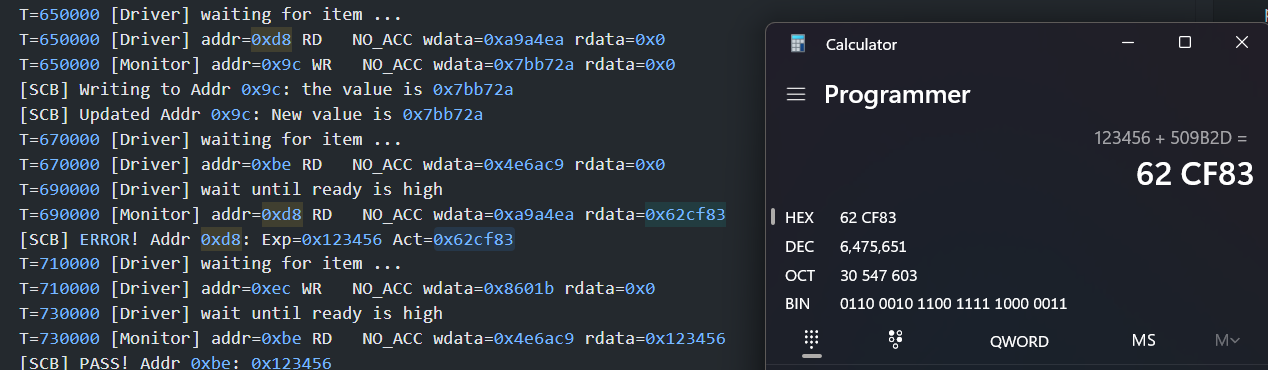
\includegraphics[width=0.8\textwidth]{acc_high_func_low_bug_2.png}
\caption{Second bug with acc=1, func=0 configuration}
\end{figure}

In contrast, when acc=0, the design operated correctly without errors:

\begin{figure}[h]
\centering
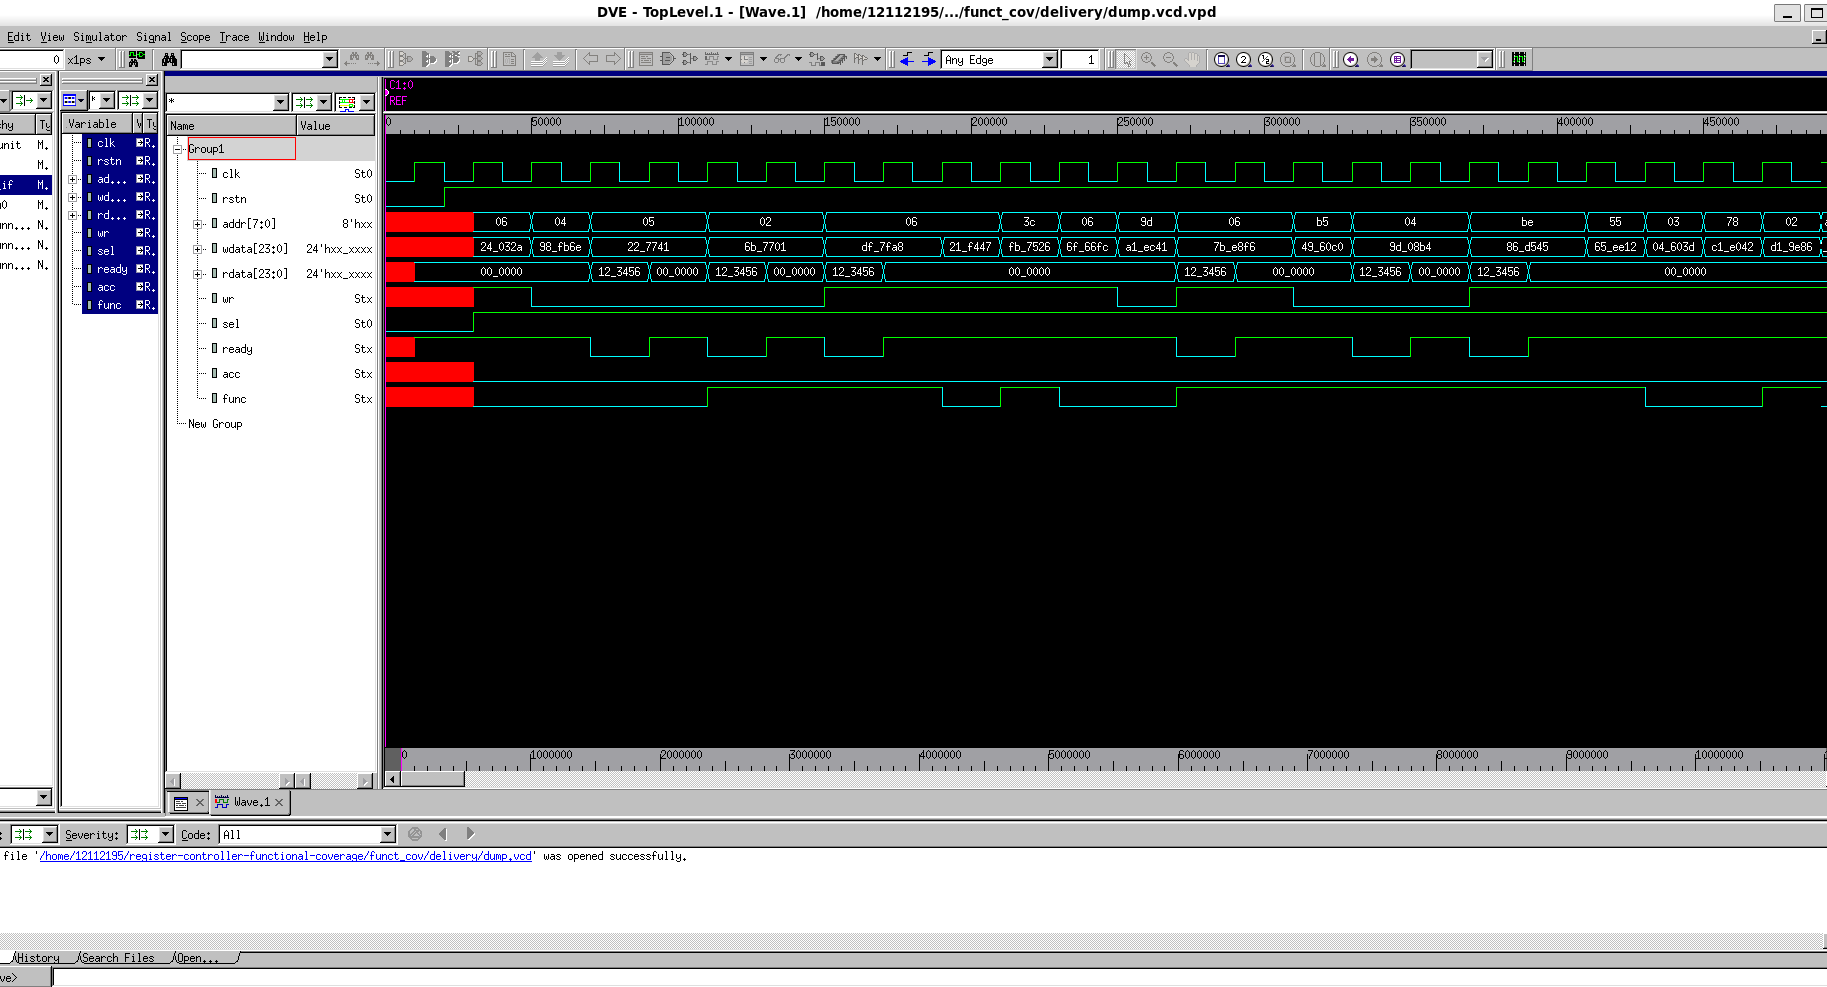
\includegraphics[width=0.8\textwidth]{acc_low_no_error.png}
\caption{Correct operation when acc=0}
\end{figure}

\textbf{Bug Fixes and Coverage Results}

After identifying and fixing the accumulate functionality bugs, comprehensive coverage analysis was performed using DVE:

\begin{figure}[h]
\centering
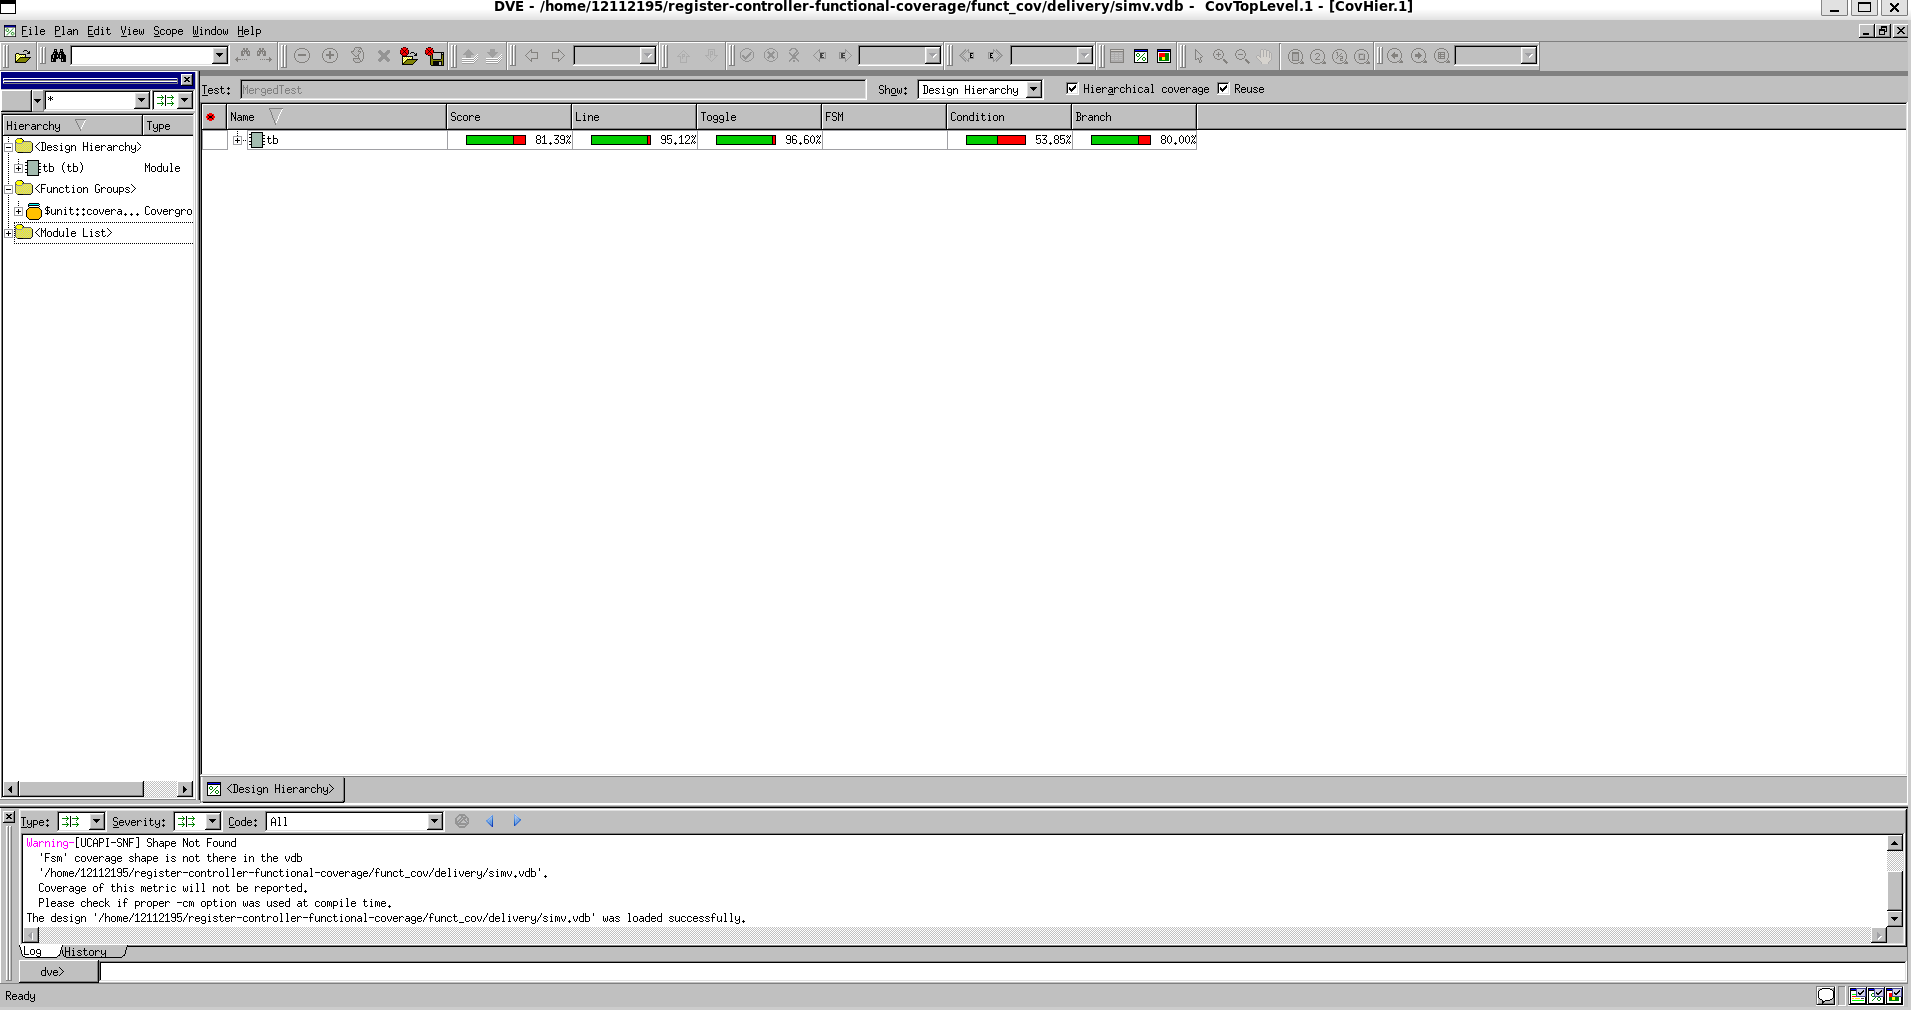
\includegraphics[width=0.8\textwidth]{code_coverage_dve_gui.png}
\caption{Code coverage analysis in DVE GUI}
\end{figure}

\begin{figure}[h]
\centering
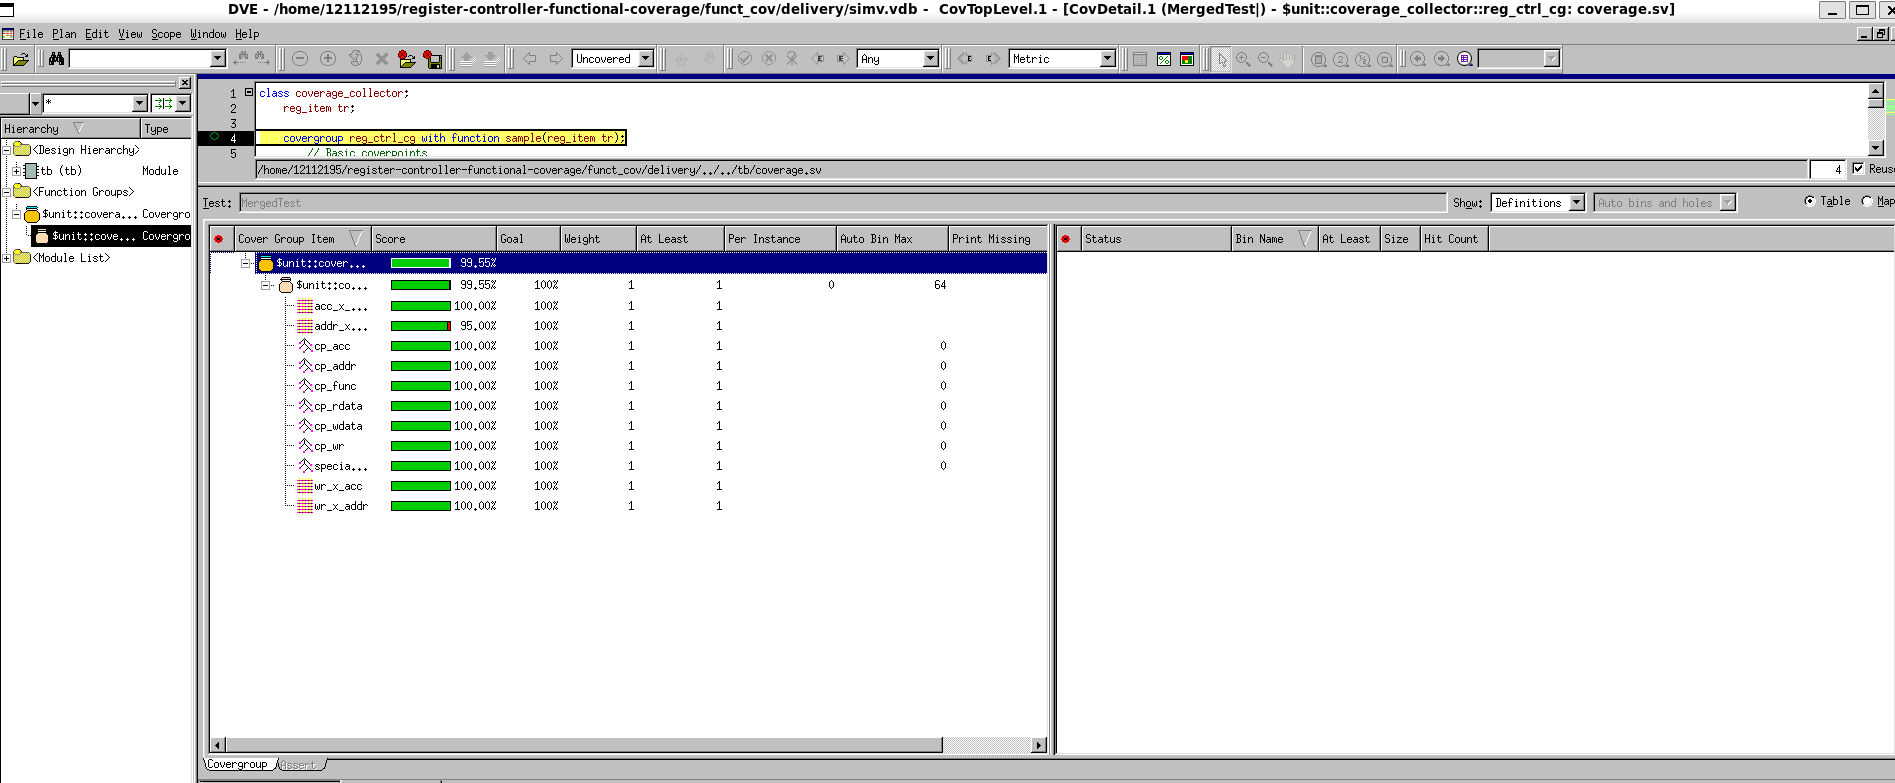
\includegraphics[width=0.8\textwidth]{functional_cov_dve_gui.png}
\caption{Functional coverage analysis in DVE GUI}
\end{figure}

Browser-based coverage reports were generated showing detailed coverage metrics:

\begin{figure}[h]
\centering
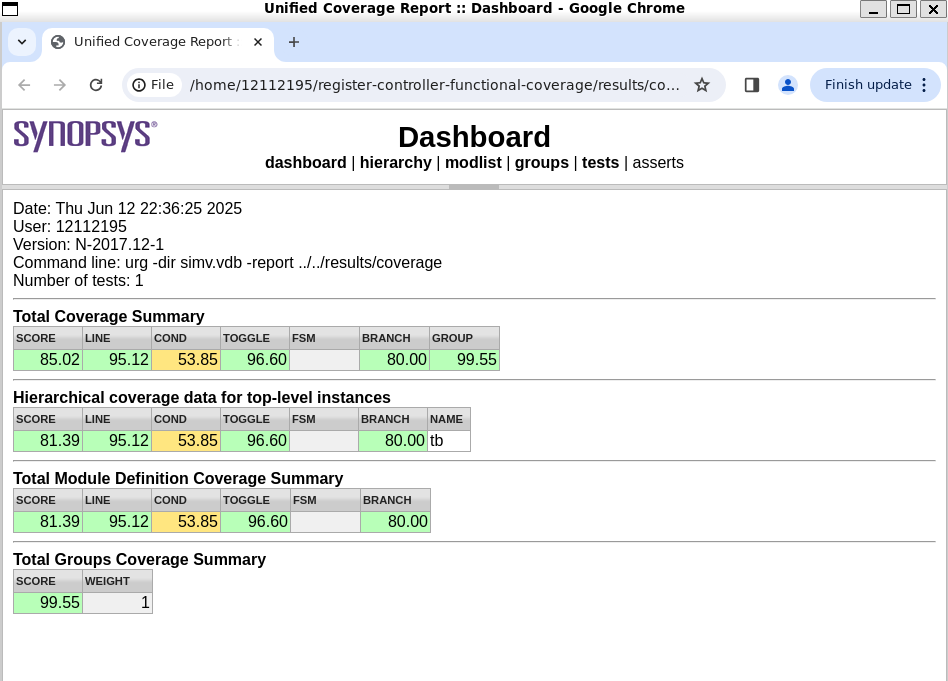
\includegraphics[width=0.8\textwidth]{browser_cov_report_overview.png}
\caption{Coverage report overview}
\end{figure}

\begin{figure}[h]
\centering
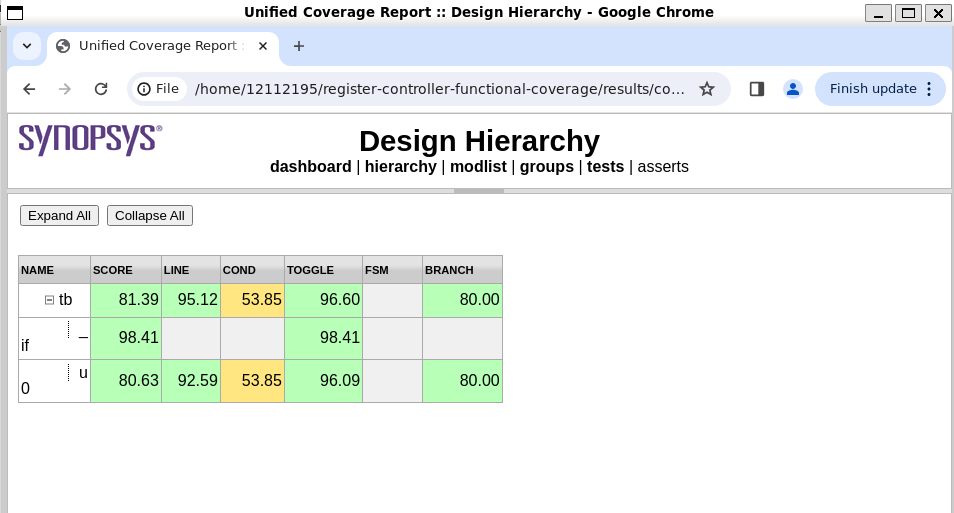
\includegraphics[width=0.8\textwidth]{browser_cov_report_hierarchy.png}
\caption{Coverage hierarchy report}
\end{figure}

\begin{figure}[h]
\centering
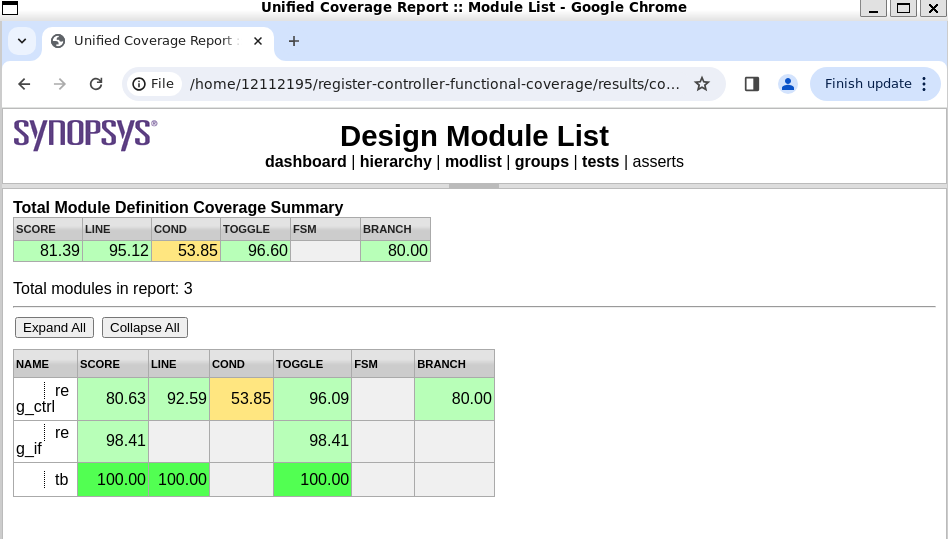
\includegraphics[width=0.8\textwidth]{browser_cov_report_design_module_list.png}
\caption{Design module coverage list}
\end{figure}

\begin{figure}[h]
\centering
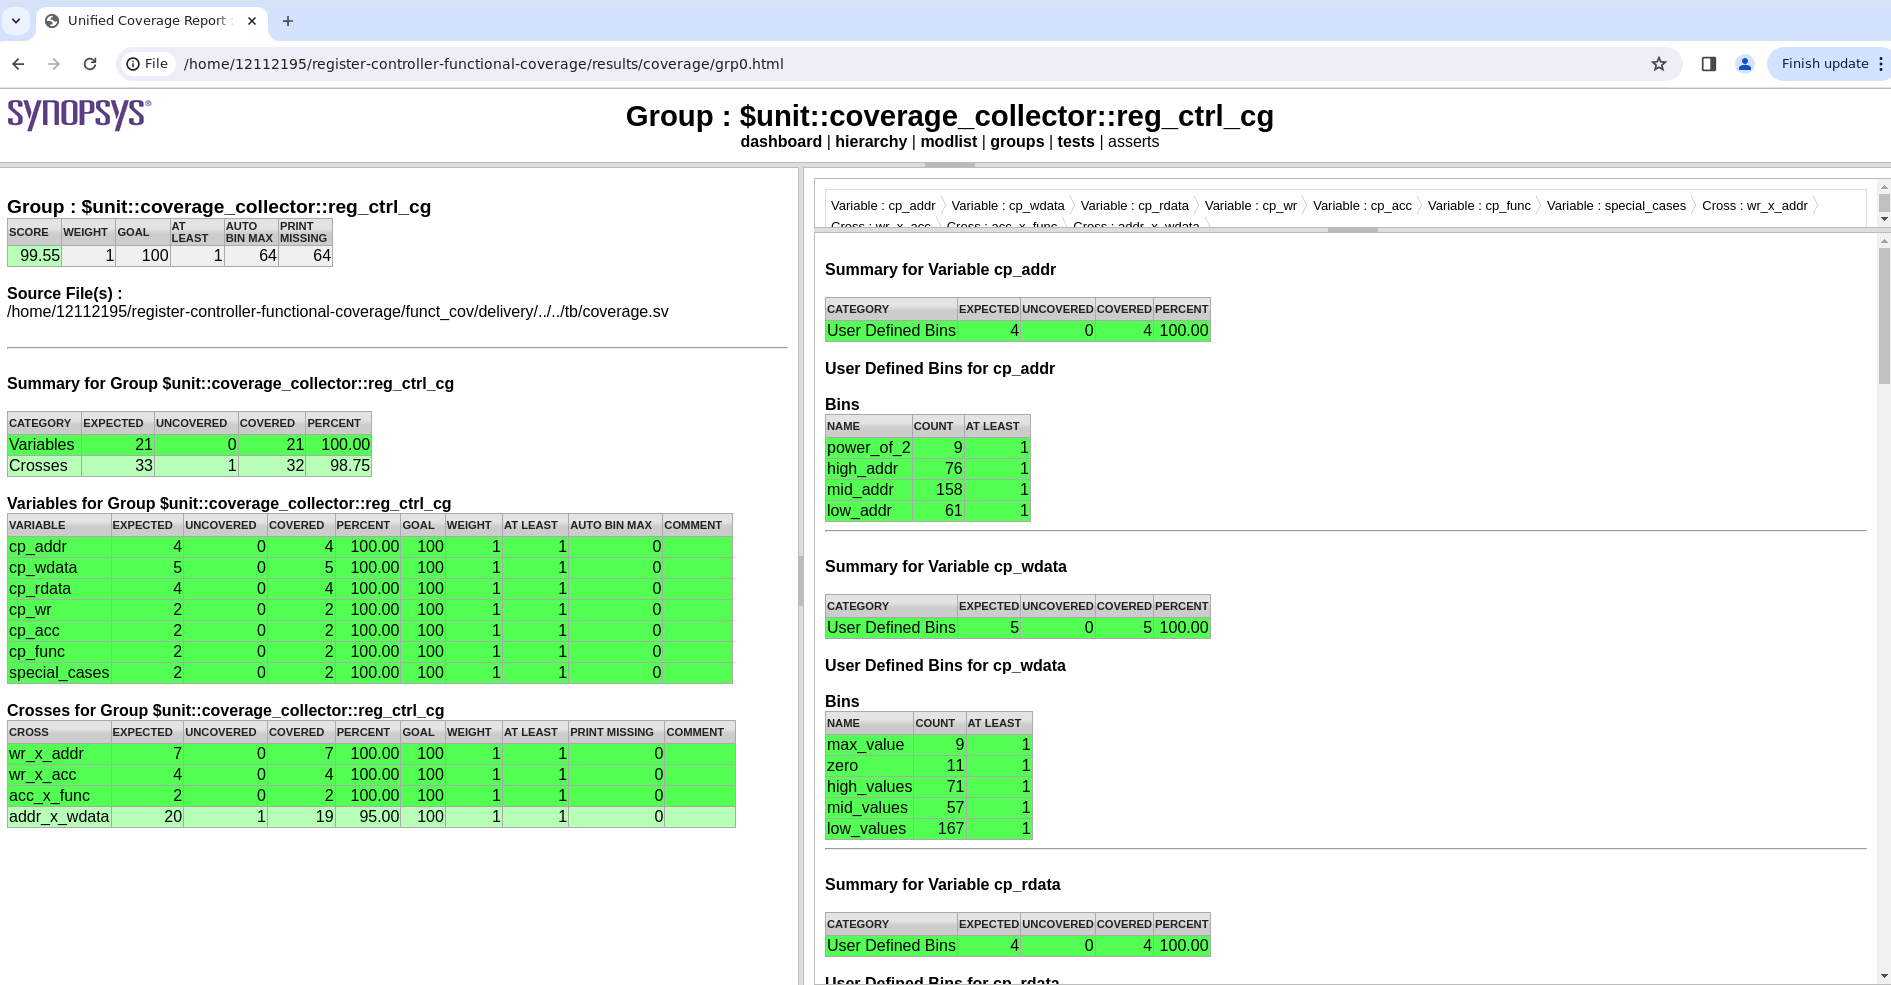
\includegraphics[width=0.8\textwidth]{browser_cov_report_group_functional_bins.png}
\caption{Functional coverage bins and cross coverage results}
\end{figure}

\textbf{Subtle Design Issue Discovery}

During a 2000-transaction test run, a subtle but concerning issue was identified where the data being written occasionally became the sum of rdata and wdata instead of the expected wdata value. This behavior occurred infrequently but was captured twice during testing:

\begin{figure}[h]
\centering
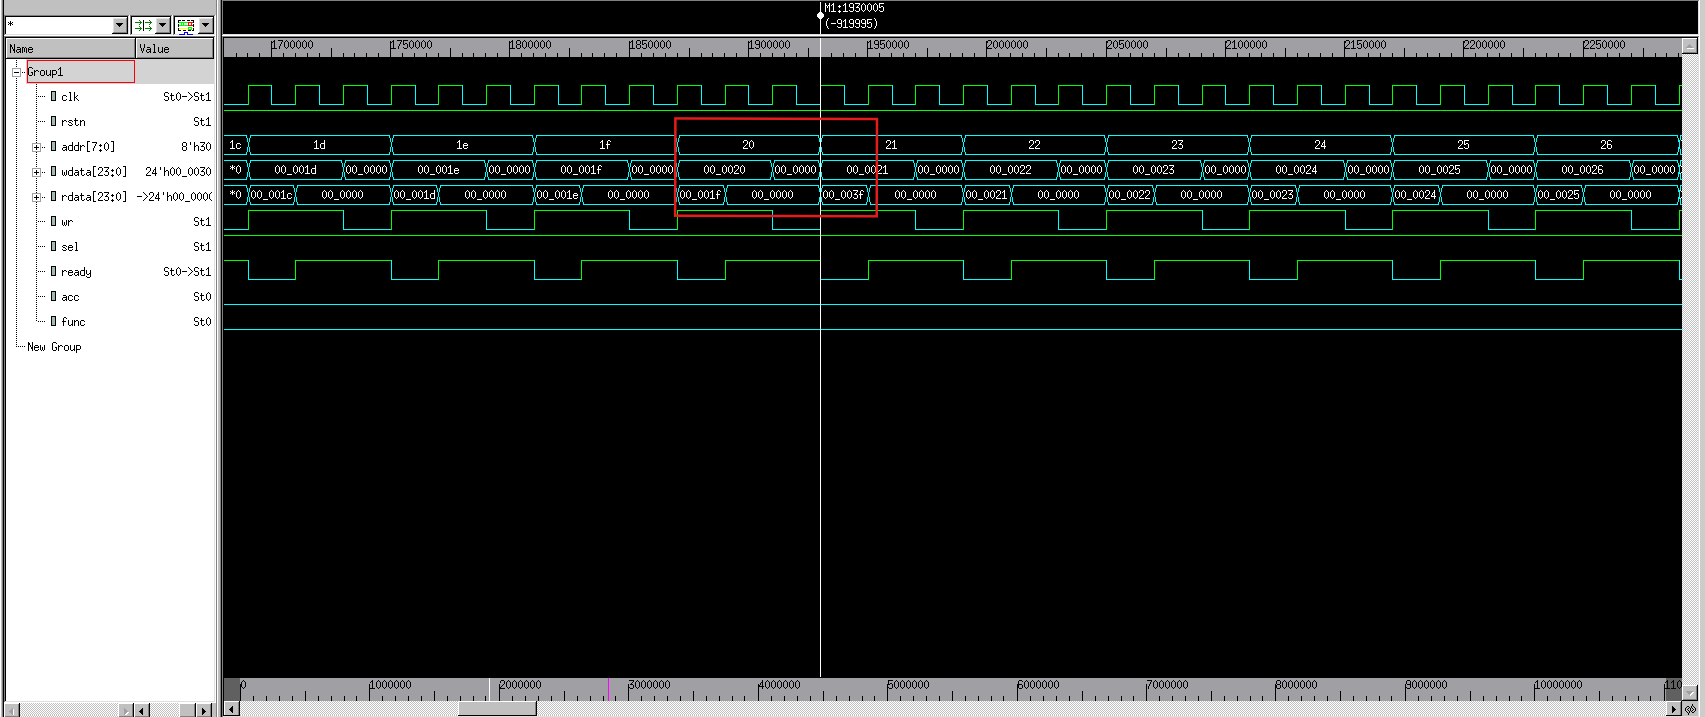
\includegraphics[width=0.8\textwidth]{weird_sum_bug_not_sure.png}
\caption{Subtle bug where written data equals rdata + wdata}
\end{figure}

This intermittent behavior suggests a potential timing or control logic issue in the design that requires further investigation, as it could lead to data corruption in production use.

\end{document}
